
%%%%%%%%%%%%%%%%%%%%%%%%%%%%%%%%%%%%%%%%%%%%%%%%%%%%%%%%%%%%%%%%%%%%%%%%

%
% Chapter 7
%

\chapter{PERFORMANCE AND DISCUSSION}
\label{chap:performance}
\section{Performance of the cooperative spectrum access system}
We assess the performance of the cooperative spectrum access system with three experiments. First, out cooperative radio runs with static interference. Second, three of our cooperative radios running together. Finally, our cooperative radio runs with other teams' radios in the DARPA Spectrum Challenge.

\subsection{Static Interference}
\label{staticInterference}
\begin{figure}[tpb]
  \begin{center}
    \centerline{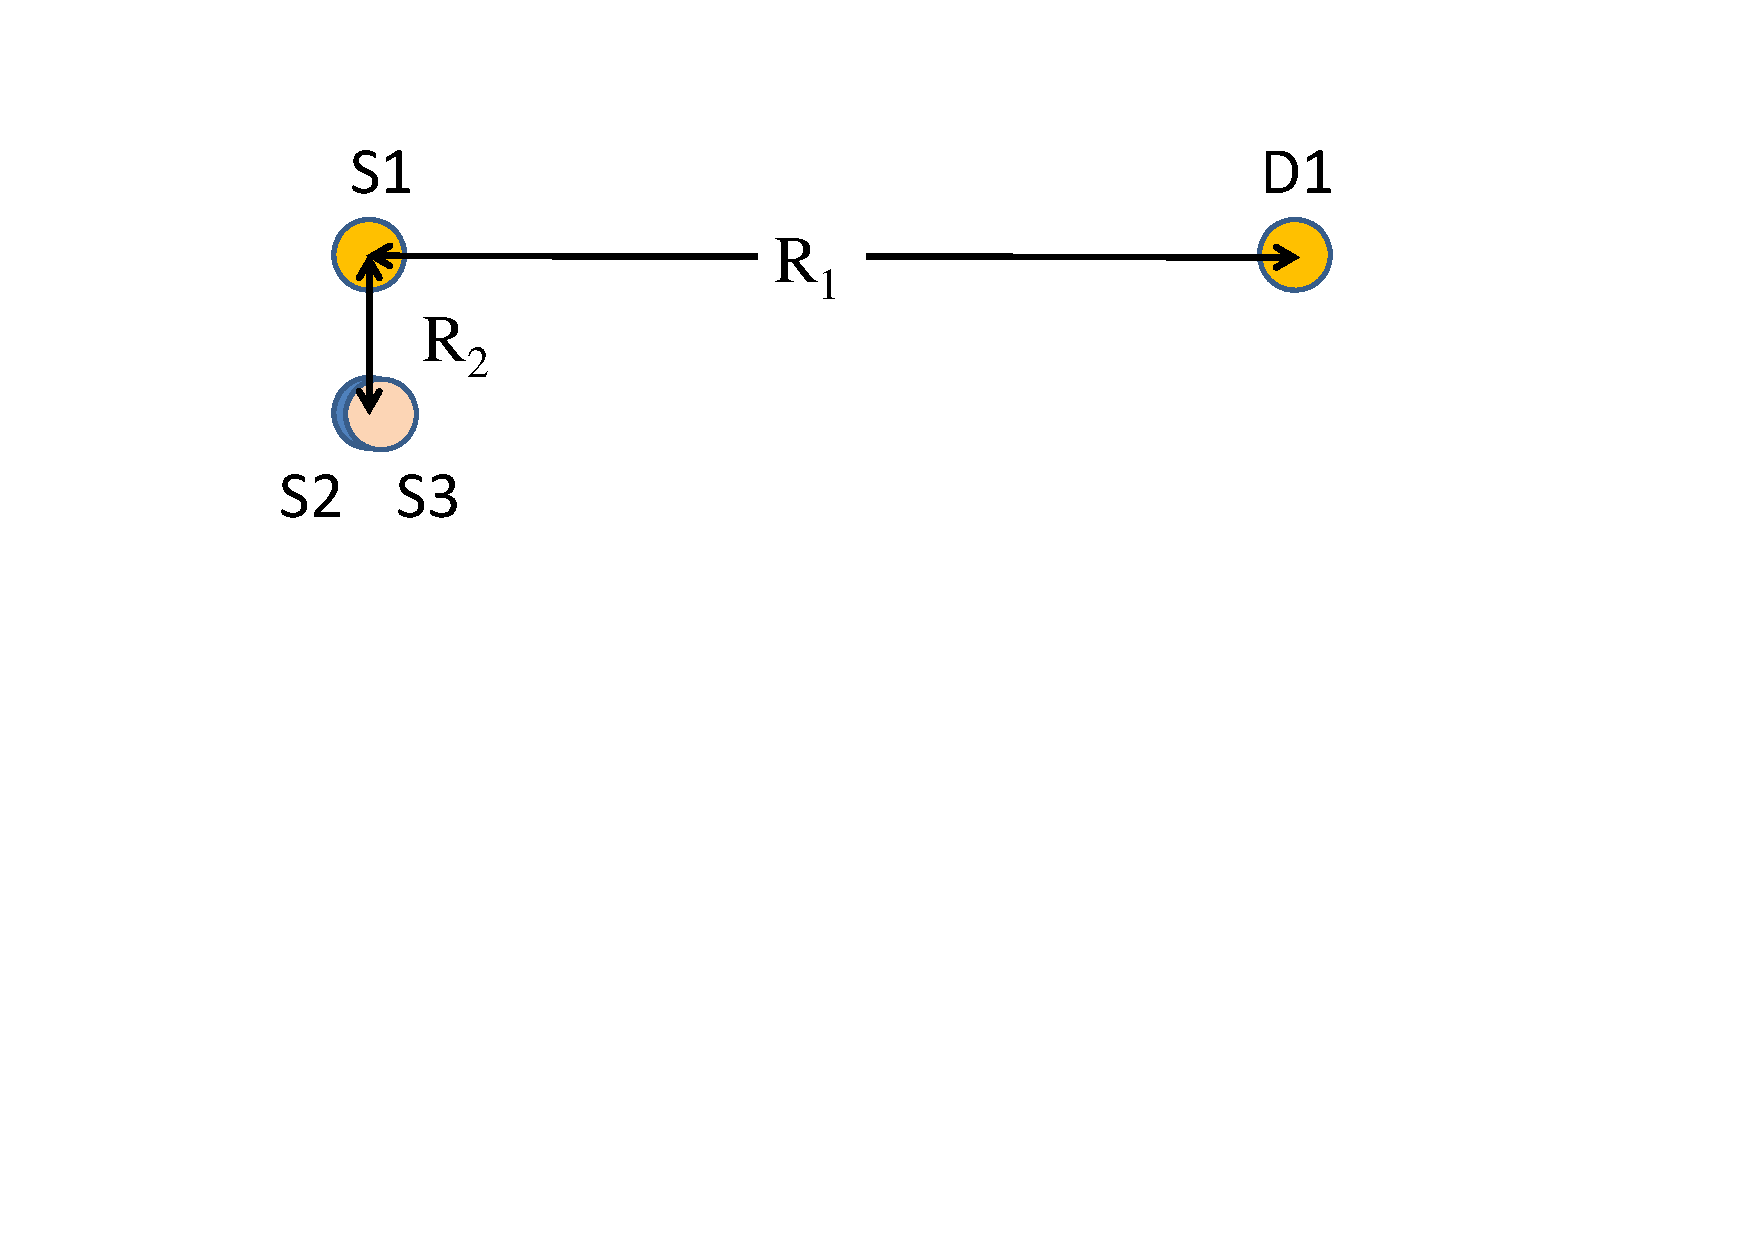
\includegraphics[width=160mm]{CoopTestNodeAssignment.pdf}}
    \caption{Radio geometry for the cooperative static interference test. The distances are roughly $R_1 = 30$ feet and $R_2 = 3$ feet}
    \label{fig:CoopTestNodeAssignment}
  \end{center}
\end{figure}

The cooperative radio is run with different types of interference, including a single-carrier signal with low-energy side lobes (SSLSL) as shown in Figure \ref{fig:SAsingleNoSideLobe}, a sinusoid tone as shown in Figure \ref{fig:SAsingleTone},  a single-carrier signal with side lobes (SSSL) as shown in Figure \ref{fig:SAsinglewithSideLob}, and a two-band signal with side lobes (TSSL) as shown in Figure \ref{fig:SAtwoSignal}.

The setup is as in Figure~\ref{fig:CoopTestNodeAssignment}. S1 is our source and D1 is our destination. S2 and S3 are the interference sources. The distance between the source and interference nodes ($R_1$) is 30 feet, and the distance between the source and destination $R_2$ is 3 feet. The distance between the source and destination is limited by the length of the Ethernet cable between the USRP and computer.

Table \ref{tbl:COOPTestResultsStatic} shows the test results. The metric is the amount of time (in seconds) for the cooperative radio to successfully transmit 15000 packets. Without interference, the average transmission time is 39.1 seconds, which is consistent with our physical layer parameters. Ideally, the transmission time with interference should be inversely proportional to the number of available sub-bands, but the test results for situation with interference are slightly worse, which suggests that there is potential improvement in the physical-layer.

\begin{table}[tpb]
\centering
    \caption{TEST RESULT (IN SECONDS): COOPERATIVE RADIO WITH STATIC INTERFERENCE (10 TESTS) \label{tbl:COOPTestResultsStatic}}
    \begin{tabular}{cccccc} \toprule
      {Test No.}
      &{No interference}
      &{\begin{tabular}{@{}l@{}} Tone\end{tabular}}
      &{\begin{tabular}{@{}l@{}} SSSL\end{tabular}}
      &{\begin{tabular}{@{}l@{}} SSLSL\end{tabular}}
      &{\begin{tabular}{@{}l@{}} TSSL\end{tabular}}   \\ \bottomrule
1                    &42.1	&46.2	&80.1	&62.7	&187.7 \\ \hline
2                    &40.9	&40.9	&78.7	&62.7	&212.0 \\ \hline
3                    &41.9	&41.2	&95.4	&59.1	&202.6 \\ \hline
4                    &38.0  &41.0	&101.1	&62.0	&193.4 \\ \hline
5                    &38.3	&42.2	&98.1	&57.5	&222.9 \\ \hline
6                    &35.9	&46.0	&82.6	&57.2	&182.6 \\ \hline
7                    &42.0	&48.8	&99.0	&57.6	&183.0 \\ \hline
8                    &38.2	&46.0	&78.8	&62.4	&182.7 \\ \hline
9                    &37.2	&46.0	&100.2	&58.9	&218.0 \\ \hline
10                   &36.1	&41.7	&93.4	&59.9	&182.2 \\\bottomrule
{\begin{tabular}{@{}c@{}} Available Number \\of sub-bands\end{tabular}}
                     &16	&15	    &12	    &12  	&7     \\ \hline
Mean                 &39.1	&44.0	&90.74	&60.0	&196.7 \\ \hline
Standard Deviation   &2.4	&2.9	&9.5	&2.3	&16.0  \\\bottomrule
    \end{tabular}
\end{table}



\subsection{Three Cooperative Radios Running Together}
\begin{table}[tpb]
  \begin{center}
    \caption{TEST RESULT (IN SECONDS): THREE COOPERATIVE RADIOS RUNNING TOGETHER (10 TESTS) \label{tbl:COOPTestResultsSelf}}
    \begin{tabular}{cc} \toprule
    {Test No.}        & {\begin{tabular}{@{}c@{}} Time to transmit \\ 15000 packets (seconds)\end{tabular}}\\ \midrule
1     &147.3\\
2     &88.9  \\
3     &132.0 \\
4     &98.0 \\
5     &115.1\\
6     &107.7\\
7     &96.4\\
8     &166.5\\
9     &110.1\\
10    &119.5\\\bottomrule
Mean                 &118.1 \\
Standard Deviation   &24.2  \\\bottomrule
    \end{tabular}
  \end{center}
\end{table}

The setup is also shown in Figure~\ref{fig:CoopTestNodeAssignment} with $R_1 = 30$ feet and $R_2 = 3$ feet. Each pair of cooperative radio is set up to use the different preambles to avoid synchronization problems. The metric is the amount of time for S1 and D1 to transmit 15000 packets. Test results are shown in Table \ref{tbl:COOPTestResultsSelf}. The average transmission time for one radio running with two other cooperative radios, is 118.1 seconds, which is almost 3 times of that without interference as shown in Table \ref{tbl:COOPTestResultsStatic}. This test result demonstrates that our cooperative radio can cooperate well with radios running the same protocol.

\subsection{Running with Other Teams' Radios}
The final test is in the Final Tournament of the DARPA Spectrum Challenge. The rules have been introduced in Chapter \ref{chap:backgound}. Our cooperative radio ranked first in the preliminary group, as show in Table \ref{tbl:COOPTestResultsDSCPreDeteils} and Table \ref{tbl:COOPTestResultsDSCPreSummary}. In the Semifinal group, our cooperative radio ranked third as shown in Table \ref{tbl:COOPTestResultsDSCSemiFinalDeteils} and Table \ref{tbl:COOPTestResultsDSCSemiFinalSummary} \cite{DSCFinalEventResults}.

\begin{table}[tpb]
  \begin{center}
    \caption{TEST RESULT: COOPERATIVE RADIO WITH OTHER TEAMS' RADIOS (PRELIMINARY ROUND DETAILS) \label{tbl:COOPTestResultsDSCPreDeteils}}
    \begin{tabular}{c lllccc} \toprule
Round  &{Player 1} &{Player 2} &{Player 3} &{P1 Score} &{P2 Score} &{P3 Score} \\ \bottomrule
1    &WSL-NEU &WINBOT &{\begin{tabular}{l} Wireless \\ Infidels\end{tabular}}      &18990  &18990  &14166 \\ \hline
2    &WINBOT  &WSL-NEU  &{\begin{tabular}{l} Notre \\Spectrum\end{tabular}}        &18703  &18703  &18271 \\ \hline
3    &{\begin{tabular}{l} Wireless \\ Infidels\end{tabular}} &{\begin{tabular}{l} Notre \\Spectrum\end{tabular}} &WINBOT &16739  &23678  &23678 \\ \hline
4    &{\begin{tabular}{l} Notre \\Spectrum\end{tabular}}      &{\begin{tabular}{l} Wireless \\ Infidels\end{tabular}} &WSL-NEU     &20633  &16627  &20633  \\ \bottomrule
    \end{tabular}
  \end{center}
\end{table}


\begin{table}[tpb]
  \begin{center}
    \caption{TEST RESULT: COOPERATIVE RADIO WITH OTHER TEAMS' RADIOS (PRELIMINARY ROUND SUMMARY) \label{tbl:COOPTestResultsDSCPreSummary}}
    \begin{tabular}{lc} \toprule
       {Group B} &{Total Score} \\ \bottomrule
WSL-NEU             &58326 \\ \hline
WINBOT              &61371 \\ \hline
Wireless Infidels   &47532 \\ \hline
Notre Spectrum      &62582  \\ \bottomrule
First:              &Notre Spectrum  \\ \hline
Second:             &WSL-NEU       \\  \bottomrule
    \end{tabular}
  \end{center}
\end{table}

\begin{table}[tpb]
  \begin{center}
    \caption{TEST RESULT: COOPERATIVE RADIO WITH OTHER TEAMS' RADIOS (SEMIFINAL ROUND DETAILS) \label{tbl:COOPTestResultsDSCSemiFinalDeteils}}
    \begin{tabular}{clllccc} \toprule
Round &{Player 1} &{Player 2} &{Player 3} &{P1 Score} &{P2 Score} &{P3 Score} \\ \bottomrule
1   &{\begin{tabular}{l} Notre \\Spectrum\end{tabular}}      &VT-Hume    &Tenn Tech  &20291  &15077  &20291 \\ \hline
2   &VT-Hume     &{\begin{tabular}{l} Notre \\Spectrum\end{tabular}}     &MarmotE        &18993  &21413  &21413 \\ \hline
3   &Tenn Tech   &MarmotE            &VT-Hume        &24471  &24471  &17912 \\ \hline
4   &MarmotE     &Tenn Tech      &{\begin{tabular}{l} Notre \\Spectrum\end{tabular}} &19597  &19597  &13877  \\ \bottomrule
    \end{tabular}
  \end{center}
\end{table}

\begin{table}[tpb]
  \begin{center}
    \caption{TEST RESULT: COOPERATIVE RADIO WITH OTHER TEAMS' RADIOS (SEMIFINAL ROUND SUMMARY) \label{tbl:COOPTestResultsDSCSemiFinalSummary}}
    \begin{tabular}{lc} \toprule
       {Group F} &{Total Score} \\ \bottomrule
Notre Spectrum  &55581 \\ \hline
VT-Hume         &51982 \\ \hline
Tenn Tech Tel   &64359 \\ \hline
MarmotE         &65481  \\ \bottomrule
First:          &MarmotE  \\ \hline
Second:         &Tenn Tech Tel      \\  \bottomrule
    \end{tabular}
  \end{center}
\end{table}

%\FloatBarrier
\section{Performance of the competitive spectrum access system}
\begin{figure}[tpb]
  \begin{center}
    \centerline{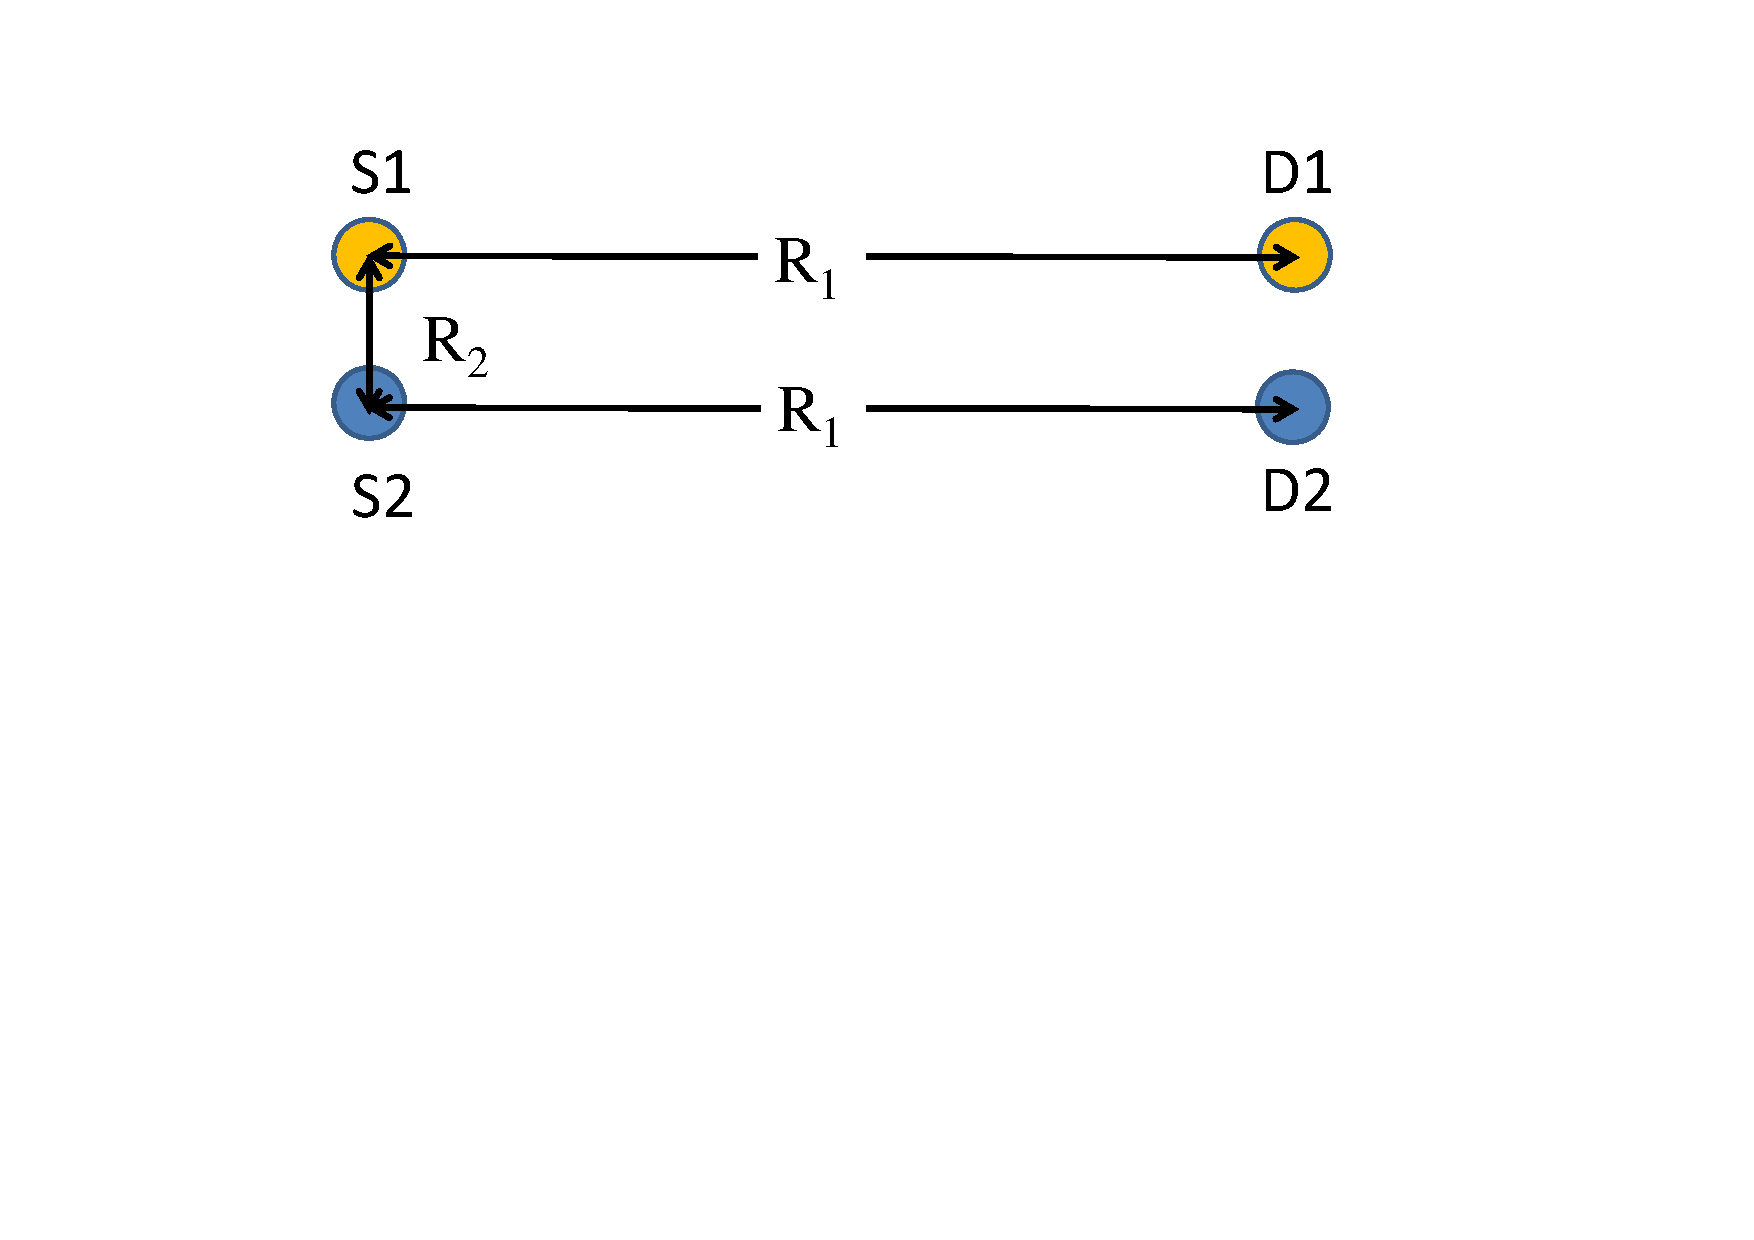
\includegraphics[width=160mm]{CompTestNodeAssignment.pdf}}
    \caption{Radio geometry for the competitive radio test. The distances are roughly $R_1 = 30$ feet and $R_2 = 3$ feet}
    \label{fig:CompTestNodeAssignment}
  \end{center}
\end{figure}

We assessed the performance of the competitive radio by running it with a pair of cooperative radios. The geometry of the set-up is shown in Figure~\ref{fig:CompTestNodeAssignment} with $R_1 = 30$ feet and $R_2 = 3$ feet. The cooperative radios are set up to transmit with a minimum number of sub-bands, which are selected as the sub-bands with the lowest energy level. Let the number of sub-bands to be used be denoted $N_{min}$. Test results are shown in Table \ref{tbl:COMPTestResultsStatic}. The metric is the amount of time (in seconds) for the competitive radio to successfully transmit 15000 packets.

In the DARPA Spectrum Challenge games, the software of our competitive radio crashed. Before it crashed, its performance was worse than some of other teams, namely Team Gator Wings and Team Wasabi \cite{DSCFinalEventResults}. Their radios occupied the same spectrum as ours, but their data could get through the interference while ours could not. 

\begin{table}[tpb]
\centering
    \caption{TEST RESULT (IN SECONDS): COMPETITIVE RADIO WITH COOPERATIVE RADIOS USING MINIMUM NUMBER OF SUB-BANDS (10 TESTS) \label{tbl:COMPTestResultsStatic}}
    \begin{tabular}{cccccc} \toprule
      {Test No.}
      &{No interference}
      &{$N_{min}=4$}
      &{$N_{min}=8$}
      &{$N_{min}=12$}  \\ \bottomrule
1	                  &33.4	&113.9	&192.7	&363.1 \\ \hline
2	                  &35.0	&136.0	&187.3	&360.5 \\ \hline
3	                  &34.1	&129.0	&189.2	&395.9 \\ \hline
4	                  &33.2	&133.3	&197.5	&363.2 \\ \hline
5	                  &33.2	&156.4	&227.2	&353.1 \\ \hline
6	                  &34.1	&136.7	&211.1	&331.5 \\ \hline
7	                  &34.0	&126.8	&206.1	&383.7 \\ \hline
8	                  &32.9	&120.5	&211.7	&362.9 \\ \hline
9	                  &33.5	&151.2	&189.3	&349.4 \\ \hline
10	                  &34.7	&139.3	&208.4	&284.0 \\ \bottomrule
Mean	              &33.8	&134.3	&202.0	&354.7 \\ \hline
Standard deviation	  &0.7	&12.9	&13.0	&30.5  \\ \bottomrule
    \end{tabular}
\end{table}

\section{Discussion}
\subsection{Observations from the Spectrum Challenge}
In the cooperative tournament, most teams utilized spectrum sensing, and a few teams performed real-time spectrum sensing. They continuously sensed even when they were transmitting on the source side. Their radios could shift almost immediately away from the spectrum where another team's signal suddenly appeared. Meanwhile, our radio sensed only once every 5 seconds and then transmitted on fixed sub-bands in one cooperative cycle. During our transmission, other teams could change their spectrum usage, resulting in spectrum conflicts.

In both competitive and cooperative games, our radio's power was less than that of many other teams' radios, even if they also used OFDM, which suggests that we still have room to optimize our power usage.

In the spectrum challenge, radios need to run on different USRPs, but the hardware of different USRPs is not exactly the same. Therefore, one parameter of the setup cannot maximize the power usage of all USRPs. Some teams calibrated their radios before a game started. For example, they would send a calibration signal sweeping across the 5 MHz bandwidth to find the best configuration of the transmission and receiving gains.

We also observed good synchronization between the transmitter and receiver. For example, Team MarmotE claimed their radios could achieve synchronization down to an SINR of -30 dB.

\subsection{Recommendations for Future Radio Design}
Real-time spectrum sensing should be developed to sense the spectrum all the time, and spectrum occupancy should be adjusted dynamically to avoid spectrum conflicts as the spectrum occupancy of other radios changes.

As discussed in the previous section, more work can be done to improve the synchronization of radios, to calibrate the radios and to increase the power usage of OFDM. Repetition codes can utilize time diversity as well as frequency diversity. The Fountain Code, Convolutional Code or Turbo Code could also be applied. The computational power of the PC is a bottleneck for channel coding because all of the signal processing is done in the PC. A PC is sufficient for a Repetition Code, Fountain Code, and Convolutional Code according to the observations of other teams as well as ours, but not for a Turbo Code. In the future, more sophisticated channel coding and signal processing techniques can be implemented in the FPGA of the USRP or a more capable SDR platform. In addition, a distributed spectrum access system with wider bandwidth can be explored.

The USRP N210 within the ORBIT testbed has two antennas. One antenna serves as a transceiver and the other is for reception only. Antenna diversity can be explored for a possible increase radio performance, as well.

Python is used for our packet management system, but we find Python has poor thread management. The threads in Python couple strongly with each other. One thread can significantly slow down the other one. In addition, as a scripting language, Python is much slower than C++. If a large amount of calculation is needed in limited time or multi-threading is necessary to deal with a significant workload, C++ is recommended instead of Python in GNU Radio.

Standard test tools and procedures should be developed for radio testing. When the radio designs are changed, the performance of radios should be measured and compared with the standards to determine if any improvement has been made. There should also be independent testers to test the radios, and developer should not responsible for the final test of their own radio components. Otherwise, errors and bugs are more likely to be hidden. A challenger is also very helpful. He or she can help the team find their weakness and look for solution to improve. During software development, good version control is also very important.

More extensively, an experiment design could be perused to determine parameters that could balance performance and robustness. Radio and network model for congested and interference-limited environment could be developed from such experimental data.
